Els codis QR (Quick Response code) són un tipus de
codis de barres de dues dimensions en forma de matriu que permet emmagatzemar informació.
La seva forma és quadrada que el caracteritza tres quadres situats a les cantonades superiors
i inferiors. Depenent a la informació que es vulgui emmagatzemar, els codis canviaran la seva
mida.

\begin{figure}[H]
    \begin{center}
      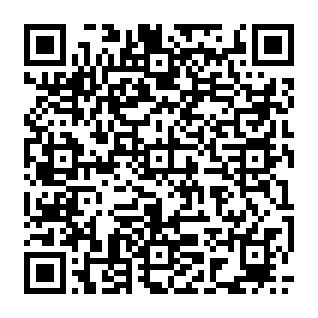
\includegraphics[scale=0.50]{Fotos/BenvingutsCodiQR.png}
    \end{center}
    \caption{Exemple d'un Codi QR}
    \label{fig:compiler_phases}
  \end{figure}

La utilització inicial dels codis QR tenia com a objectiu principal en la indústria de l'automoció.
Actualment, la possibilitat de llegir els codis QR és existent, ja sigui amb el telèfon mòbil que ens permet l'ús d'aquests
codis en una infinitat d'aplicacions. Una de les raons principals són perquè aquests codis poden interactuar fàcilment amb
un dispositiu mòbil i realitzar accions. En l'actualitat, a causa de la Covid-19, s'ha fet ús d'aquesta eina per poder-nos
descarregar o en la lectura d'un codi QR, llegir una URL d'una pàgina web per descarregar-nos la carta o el menú d'un restaurant.

\subsubsection{Estructura Codi QR}

En aquest subapartat es fa referència a l'estructura i les especificacions del codi QR.

\begin{itemize}
  \item \emph{Marques d'orientació}: A dins d'aquestes marques podem trobar els patrons de posició i els d'alineació.
  Estan situades als extrems del codi QR. S'utilitzen per saber l'orientació del codi.
  Poden variar depenent de la dimensió del codi QR.
    \begin{itemize}
      \item \emph{Patrons de posició}: Són tres quadrats que estan als extrems del codi QR.
      \item \emph{patrons d'alineació}: S'usa per a la detecció de la posició.
    \end{itemize}
  \item \emph{Informació del format}: S'empra per saber quin nivell d'error i quina màscara s'ha aplicat en el codi.
  \item \emph{Mètrica}: Igual a tots els codis QR i és feta servir per identificar els punts blancs i negres de la matriu.
  \item \emph{Dades}: Les dades s'emmagatzemen en codewords de mòduls. Els codewords són conjunts de 8 bits que varien la seva forma.
  N'hi ha de dos tipus, el d'informació i el de correcció d'errors. Les dades que hi ha tenen uns bits dedicats a especificar
  el format de les dades, i la quantitat de caràcters que hi ha en el QR. Actualment, els QR accepten diferents formats per les dades.
  \item \emph{Codis correcció d'errors}: Proporcionen la capacitat de correcció dels codis QR, que s'expressa en un percentatge i correspon
  al tant per cent de dades que es podrà recuperar en cas d'error. Actualment, hi ha 4 nivells de correcció pels codis QR:
  \begin{itemize}
    \item L 7\%
    \item M 15\%
    \item Q 25\%
    \item H 30\%
  \end{itemize}
  \item \emph{Informació de la versió}: Conté la informació de la versió que s'està fent servir. Situada en els laterals
  de dins de les marques d'orientació.
  \item \emph{Sense ús}: Es troben en algunes versions dels codis QR, l'últim codeword dels codis d'error no es fa servir.
\end{itemize}

\begin{figure}[H]
    \begin{center}
      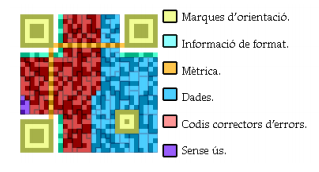
\includegraphics[scale=1]{Fotos/EstructuraCodiQR.png}
    \end{center}
    \caption{Estructura dels Codis QR}
    \label{fig:compiler_phases}
  \end{figure}

\subsubsection{Generar Codi QR}

En aquest projecte l'encarregat de fer el codi QR i mostrar-lo als usuaris és el \emph{front-end} de l'aplicació. Encara que
l'encarregat de generar el text és el servidor. \autoref{chap:back-end}

\subsubsection{Lectura Codi QR}


En aquest projecte l'encarregat de fer la lectura del QR és la Raspberry Pi actuant com a barrera fent servir una càmera.
\autoref{chap:raspberryPi}